%%%%%%%%%%%%%%%%%%%%%%%%%%%%%%%%%%%%%%%%%%%%%%%%%%%%%%%%%%%%%%%%%%%%%%%%%%%%%%%%%%
\begin{frame}[fragile]\frametitle{}
\begin{center}
{\Large Teaching Skills }
\end{center}
\end{frame}

%%%%%%%%%%%%%%%%%%%%%%%%%%%%%%%%%%%%%%%%%%%%%%%%%%%%%%%%%%%
\begin{frame}[fragile]\frametitle{Syllabus}

\begin{itemize}
\item  Essentials  of  good  lesson  plan:  concepts,  needs,  planning  of  teaching  Yoga  (Shatkriya, Asana, Pranayama \& practices leading to Dhyana) 
\item  Principles  of  teaching  Yoga  protocol  to  different  groups  (beginners,  children,  youth, women, Geriatric population, and special attention group). 
\item  Preparation for a Yoga class (before and during the class) 
\item  Factors influencing yoga teaching. 
\item  Class management in Yoga: its meaning and needs. 
\item  Conducting yoga practical lessons: Precautions \& Contraindications of practices)  
\item  Salient features of Ideal Yoga Instructor.  
\item  Models of ideal Yoga lesson plans 
\end{itemize}
\end{frame}

%%%%%%%%%%%%%%%%%%%%%%%%%%%%%%%%%%%%%%%%%%%%%%%%%%%%%%%%%%%%%%%%%%%%%%%%%%%%%%%%%%
\begin{frame}[fragile]\frametitle{}
\begin{center}
{\Large Introduction}
\end{center}
\end{frame}

%%%%%%%%%%%%%%%%%%%%%%%%%%%%%%%%%%%%%%%%%%%%%%%%%%%%%%%%%%%
\begin{frame}[fragile]\frametitle{Benefits of Teaching Yoga}
      \begin{itemize}
          \item Teaching yoga benefits both the teacher and the learners.
          \item Contributes to learners' good health and ultimate happiness.
          \item Yoga instructors can experience personal growth.
          \item Many opportunities exist for yoga professionals in various settings.
      \end{itemize}
\end{frame}

%%%%%%%%%%%%%%%%%%%%%%%%%%%%%%%%%%%%%%%%%%%%%%%%%%%%%%%%%%%
\begin{frame}[fragile]\frametitle{Principles of Effective Yoga Teaching}
      \begin{itemize}
          \item Activity and experience are crucial for learning.
          \item Correct practice is essential for skill-learning.
          \item Observing enhances attention, awareness, and skilful action.
          \item Visual demonstrations are effective for learning motor skills.
          \item Effective teaching depends on knowledge of various principles.
      \end{itemize}
\end{frame}

%%%%%%%%%%%%%%%%%%%%%%%%%%%%%%%%%%%%%%%%%%%%%%%%%%%%%%%%%%%
\begin{frame}[fragile]\frametitle{Teaching Methods in Yoga}
      \begin{itemize}
          \item The lecture method is beneficial when combined with other methods.
          \item Visual materials help students retain lecture content.
          \item Response-to-instruction method ensures uniform student responses.
          \item Project method enables practical application of learned skills.
          \item Group settings cater to varied and deeper yoga practice experiences.
      \end{itemize}
\end{frame}

%%%%%%%%%%%%%%%%%%%%%%%%%%%%%%%%%%%%%%%%%%%%%%%%%%%%%%%%%%%
\begin{frame}[fragile]\frametitle{Modern Challenges and Expectations in Yoga Teaching}
      \begin{itemize}
          \item Advances in science have altered communication systems.
          \item Technology reduces the need for manpower in teaching.
          \item Teachers should know more than students and be prepared to answer questions.
          \item If unsure, teachers should commit to finding answers and explaining later.
      \end{itemize}
\end{frame}



%%%%%%%%%%%%%%%%%%%%%%%%%%%%%%%%%%%%%%%%%%%%%%%%%%%%%%%%%%%%%%%%%%%%%%%%%%%%%%%%%%
\begin{frame}[fragile]\frametitle{}
\begin{center}
{\Large Essentials  of  good  lesson  plan:  concepts,  needs,  planning  of  teaching  Yoga  (Shatkriya, Asana, Pranayama \& practices leading to Dhyana) }
\end{center}
\end{frame}

%%%%%%%%%%%%%%%%%%%%%%%%%%%%%%%%%%%%%%%%%%%%%%%%%%%%%%%%%%%
\begin{frame}[fragile]\frametitle{Essentials of Good Lesson Plan}
\begin{columns}
    \begin{column}[T]{0.5\linewidth}
      \begin{itemize}
        \item \textbf{Concepts}: Clearly define \textbf{objectives} for \textbf{Shatkriya}, \textbf{Asana}, \textbf{Pranayama}, and \textbf{Dhyana}.
        \item \textbf{Needs Assessment}: Identify \textbf{student needs} and \textbf{levels} of experience.
        \item \textbf{Structure}: Organize \textbf{class flow} with \textbf{warm-up}, \textbf{practice}, and \textbf{cool-down}.
        \item \textbf{Timing}: Allocate \textbf{appropriate time} for each \textbf{segment}.
        \item \textbf{Flexibility}: Be \textbf{adaptive} to \textbf{student feedback} and \textbf{progress}.
      \end{itemize}
    \end{column}
    \begin{column}[T]{0.5\linewidth}
        \begin{center}
        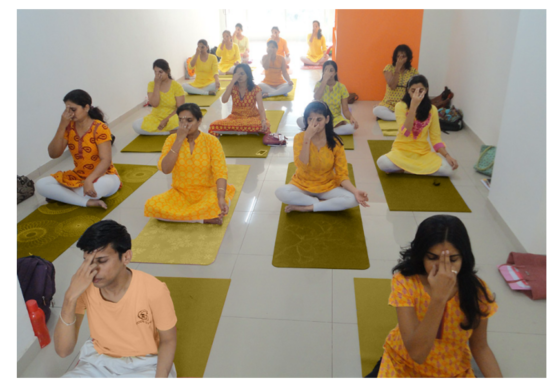
\includegraphics[width=\linewidth,keepaspectratio]{ycb1_teaching_demo}
		
		{\tiny (Ref: Certification  of Yoga Professionals Official Guidebook For Level I (Instructor))}		
        \end{center}	
    \end{column}
\end{columns}
\end{frame}


%%%%%%%%%%%%%%%%%%%%%%%%%%%%%%%%%%%%%%%%%%%%%%%%%%%%%%%%%%%%%%%%%%%%%%%%%%%%%%%%%%
\begin{frame}[fragile]\frametitle{}
\begin{center}
{\Large Principles  of  teaching  Yoga  protocol  to  different  groups  (beginners,  children,  youth, women, Geriatric population, and special attention group)}
\end{center}
\end{frame}

%%%%%%%%%%%%%%%%%%%%%%%%%%%%%%%%%%%%%%%%%%%%%%%%%%%%%%%%%%%
\begin{frame}[fragile]\frametitle{Principles of Teaching Yoga Protocol to Different Groups}
\begin{columns}
    \begin{column}[T]{0.5\linewidth}
      \begin{itemize}
        \item \textbf{Beginners}: Use \textbf{simple} instructions and \textbf{basic poses}.
        \item \textbf{Children}: Include \textbf{fun} and \textbf{interactive} elements.
        \item \textbf{Youth}: Emphasize \textbf{strength} and \textbf{endurance}.
        \item \textbf{Women}: Adapt for \textbf{pregnancy} and \textbf{menstruation}.
        \item \textbf{Geriatric Population}: Focus on \textbf{gentle} movements and \textbf{balance}.
        \item \textbf{Special Attention Group}: Customize for \textbf{health conditions} and \textbf{physical limitations}.
      \end{itemize}
    \end{column}
    \begin{column}[T]{0.5\linewidth}
        \begin{center}
        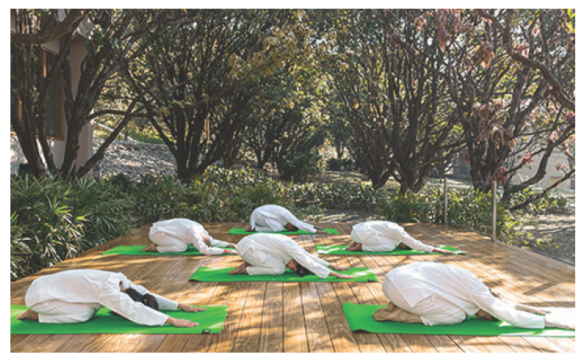
\includegraphics[width=\linewidth,keepaspectratio]{ycb1_teaching_group}
		
		{\tiny (Ref: Certification  of Yoga Professionals Official Guidebook For Level I (Instructor))}		
        \end{center}	
    \end{column}
\end{columns}
\end{frame}


%%%%%%%%%%%%%%%%%%%%%%%%%%%%%%%%%%%%%%%%%%%%%%%%%%%%%%%%%%%%%%%%%%%%%%%%%%%%%%%%%%
\begin{frame}[fragile]\frametitle{}
\begin{center}
{\Large Preparation for a Yoga class (before and during the class)}
\end{center}
\end{frame}

%%%%%%%%%%%%%%%%%%%%%%%%%%%%%%%%%%%%%%%%%%%%%%%%%%%%%%%%%%%
\begin{frame}[fragile]\frametitle{Preparation for a Yoga Class (Before and During)}
\begin{columns}
    \begin{column}[T]{0.5\linewidth}
      \begin{itemize}
        \item \textbf{Pre-Class Planning}: Develop a \textbf{lesson plan} and \textbf{set goals}.
        \item \textbf{Set Up Space}: Arrange \textbf{props} and \textbf{equipment} for \textbf{class}.
        \item \textbf{Check Equipment}: Ensure all \textbf{yoga mats} and \textbf{tools} are \textbf{clean} and \textbf{functional}.
        \item \textbf{Greet Students}: Welcome students and \textbf{address} any \textbf{individual needs}.
        \item \textbf{Monitor Flow}: Adjust the \textbf{class} as needed based on \textbf{student feedback} and \textbf{progress}.
      \end{itemize}
    \end{column}
    \begin{column}[T]{0.5\linewidth}
        \begin{center}
        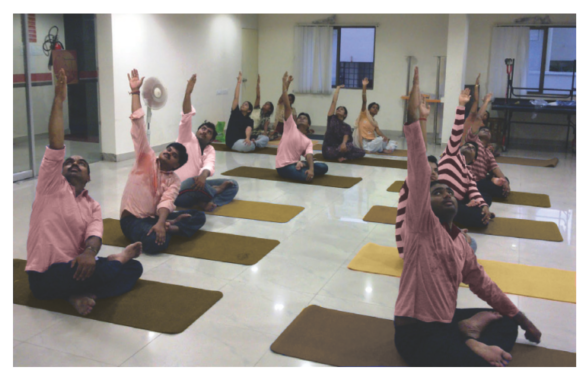
\includegraphics[width=\linewidth,keepaspectratio]{ycb1_teaching_prep}
		
		{\tiny (Ref: Certification  of Yoga Professionals Official Guidebook For Level I (Instructor))}	
        \end{center}	
    \end{column}
\end{columns}
\end{frame}


%%%%%%%%%%%%%%%%%%%%%%%%%%%%%%%%%%%%%%%%%%%%%%%%%%%%%%%%%%%%%%%%%%%%%%%%%%%%%%%%%%
\begin{frame}[fragile]\frametitle{}
\begin{center}
{\Large Conducting yoga practical lessons: Precautions \& Contraindications of practices}
\end{center}
\end{frame}

%%%%%%%%%%%%%%%%%%%%%%%%%%%%%%%%%%%%%%%%%%%%%%%%%%%%%%%%%%%
\begin{frame}[fragile]\frametitle{Conducting Yoga Practical Lessons: Precautions \& Contraindications}
\begin{columns}
    \begin{column}[T]{0.5\linewidth}
      \begin{itemize}
        \item \textbf{Assess Individual Needs}: Evaluate \textbf{health conditions} and \textbf{physical limitations}.
        \item \textbf{Modify Poses}: Adapt \textbf{asanas} to suit \textbf{individual needs}.
        \item \textbf{Monitor Students}: Watch for \textbf{discomfort} or \textbf{strain}.
        \item \textbf{Avoid Overexertion}: Prevent \textbf{overexertion} and \textbf{injuries}.
        \item \textbf{Educate on Contraindications}: Inform about \textbf{contraindications} for specific \textbf{conditions}.
      \end{itemize}
    \end{column}
    \begin{column}[T]{0.5\linewidth}
        \begin{center}
        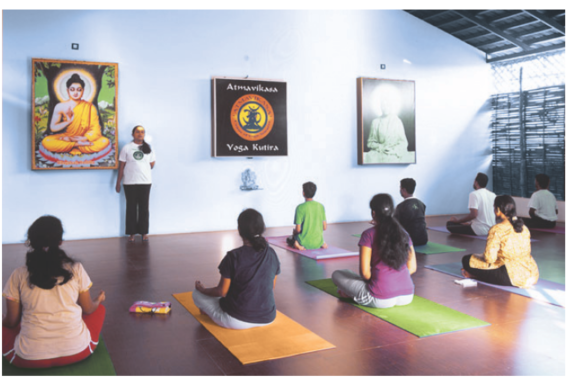
\includegraphics[width=\linewidth,keepaspectratio]{ycb1_teaching_lecture}
		
		{\tiny (Ref: Certification  of Yoga Professionals Official Guidebook For Level I (Instructor))}	
        \end{center}	
    \end{column}
\end{columns}
\end{frame}


%%%%%%%%%%%%%%%%%%%%%%%%%%%%%%%%%%%%%%%%%%%%%%%%%%%%%%%%%%%%%%%%%%%%%%%%%%%%%%%%%%
\begin{frame}[fragile]\frametitle{}
\begin{center}
{\Large Salient features of Ideal Yoga Instructor}
\end{center}
\end{frame}

%%%%%%%%%%%%%%%%%%%%%%%%%%%%%%%%%%%%%%%%%%%%%%%%%%%%%%%%%%%
\begin{frame}[fragile]\frametitle{Salient Features of an Ideal Yoga Instructor}
\begin{columns}
    \begin{column}[T]{0.5\linewidth}
      \begin{itemize}
        \item \textbf{Knowledgeable}: Deep understanding of \textbf{yoga principles} and \textbf{practices}.
        \item \textbf{Communicative}: Clear and \textbf{effective communication} skills.
        \item \textbf{Empathetic}: Ability to \textbf{understand} and \textbf{address student needs}.
        \item \textbf{Professional}: Maintains \textbf{professionalism} and \textbf{ethics}.
        \item \textbf{Adaptable}: Flexible in \textbf{teaching methods} and \textbf{lesson plans}.
      \end{itemize}
    \end{column}
    \begin{column}[T]{0.5\linewidth}
        \begin{center}
        
\includegraphics[width=\linewidth,keepaspectratio]{ycb1_teaching_teacher}
		
		{\tiny (Ref: Certification  of Yoga Professionals Official Guidebook For Level I (Instructor))}	
        \end{center}	
    \end{column}
\end{columns}
\end{frame}


%%%%%%%%%%%%%%%%%%%%%%%%%%%%%%%%%%%%%%%%%%%%%%%%%%%%%%%%%%%%%%%%%%%%%%%%%%%%%%%%%%
\begin{frame}[fragile]\frametitle{}
\begin{center}
{\Large Models of ideal Yoga lesson plans}
\end{center}
\end{frame}

%%%%%%%%%%%%%%%%%%%%%%%%%%%%%%%%%%%%%%%%%%%%%%%%%%%%%%%%%%%
\begin{frame}[fragile]\frametitle{Models of Ideal Yoga Lesson Plans}
\begin{columns}
    \begin{column}[T]{0.5\linewidth}
      \begin{itemize}
        \item \textbf{Structured Flow}: Follow a \textbf{logical sequence} of \textbf{warm-up}, \textbf{practice}, and \textbf{cool-down}.
        \item \textbf{Objective Focused}: Align \textbf{objectives} with \textbf{student needs} and \textbf{goals}.
        \item \textbf{Time Management}: Allocate \textbf{time} for each \textbf{segment} of the lesson.
        \item \textbf{Variety}: Incorporate a \textbf{variety} of \textbf{asanas}, \textbf{pranayama}, and \textbf{meditation}.
        \item \textbf{Flexibility}: Be \textbf{flexible} to \textbf{adapt} to \textbf{student feedback}.
      \end{itemize}
    \end{column}
    \begin{column}[T]{0.5\linewidth}
        \begin{center}
        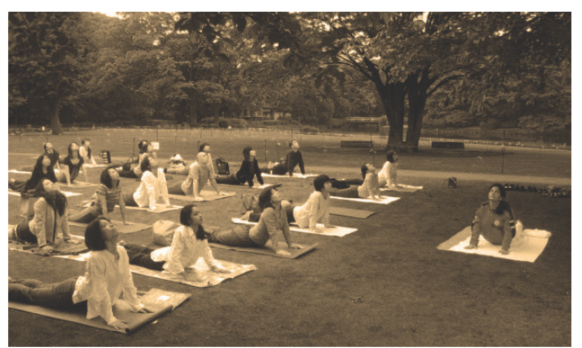
\includegraphics[width=\linewidth,keepaspectratio]{ycb1_teaching_lesson}
		
		{\tiny (Ref: Certification  of Yoga Professionals Official Guidebook For Level I (Instructor))}	
        \end{center}	
    \end{column}
\end{columns}
\end{frame}

